\chapter{Prototipo 1}
  \section{Análisis}
    \subsection{Objetivo}
      Crear el módulo de conexión de datos apropiado para el manejo de la información de acuerdo a un modelo de datos propuesto diseñado por el equipo de trabajo.

    \subsection{Características}
      \begin{itemize}
        \item El modelo de datos propuesto deberá satisfacer las necesidades para trabajar con diferentes artículos y la interacción con sus usuarios.
        \item El sistema deberá permitir la conexión a la fuente de datos que corresponda con el modelo propuesto.
        \item El sistema deberá ser capaz de realizar operaciones sobre los datos de la fuente para el correcto funcionamiento de los procesos lógicos del sistema.
      \end{itemize}

    \subsection{Restricciones}
      \begin{itemize}
        \item El sistema se verá limitado por el lenguaje de desarrollo Java.
        \item Para el caso de estudio, el sistema operará con el gestor de base de dato propio de Neo4j. 
      \end{itemize}

  \section{Diseño}
    \subsection{Modelo de datos}
      Para la API, el problema fundamental recae en que las recomendaciones pueden ser utilizadas para diversos casos de estudio, buscando una generalización de las características mínimas requeridas para realizar recomendaciones se plantea un modelo de datos utilizando tres principales entidades: Usuarios, Artículos a recomendar, y Categorías como características que permitan clasificar los diferentes artículos. La información que será guardada y posteriormente consultada por otros módulos del sistema seguirá un esquema propuesto por el equipo de trabajo, éste recopila la estructura de evaluaciones básicas generadas en prácticamente cualquier tipo de artículos, películas, platillos, libros, entre otros como podemos ver en el siguiente diagrama de grafos.

      \newpage
          \begin{landscape}
            \begin{figure}[h!]
            \centering
            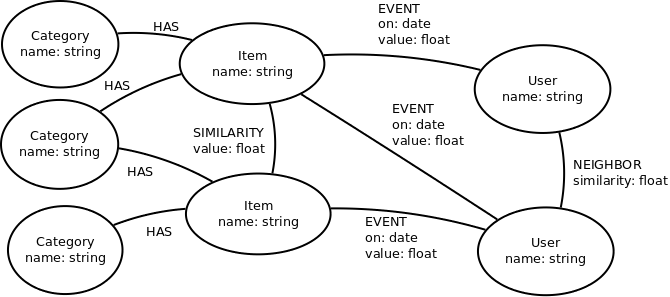
\includegraphics[width=22.5cm,height=12cm]{./images/general_data_model.png}
            \caption{Modelo general necesario para el manejo de la información}
          \end{figure}
          \end{landscape}
        \newpage

      Dentro del modelo de la aplicación final se toma en cuenta el modelo general mínimo necesario para trabajar la información añadiendo información relevante sobre el caso de estudio que recae en platillos como articulos a recomendar. Considerando al final las siguientes entidades.
      \begin{itemize}
        \item Platillos
        \item Usuarios
        \item Restaurantes
        \item Categorías
      \end{itemize}

      Para la información de los restaurantes, el modelo  permitirá almacenar como atributo una fuente de información externa en caso de ser utilizada, para obtener datos adicionales a los que se poseen en la base de datos como pueden ser los contenidos almacenados por Foursquare en su API para la búsqueda de restaurantes.

      Las relaciones posibles entre los elementos Usuario, Restaurante, Platillo y sus posibles Categorías son visualizados en el siguiente diagrama.

      \newpage
      \begin{landscape}
        \begin{figure}[h!]
          \centering
          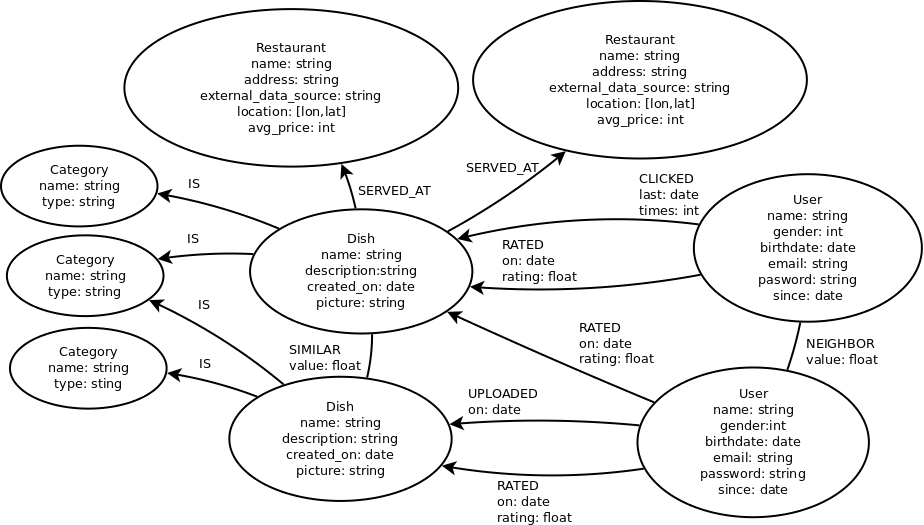
\includegraphics[width=22.5cm,height=12cm]{./images/sc_data_model.png}
          \caption{Modelo de datos propuesto para el caso de estudio}
        \end{figure}
      \end{landscape}
      \newpage

      Como se puede observar en el diagrama previo, los nodos del grafo corresponden a las entidades Usuario, Platillo, Restaurante y Categoría. Donde las relaciones entre ellos se describen de la siguiente manera: 
      \begin{itemize}
        \item Un platillo puede ser de una o más categorías.
        \item Un platillo puede ser servido en uno o más restaurantes
        \item Un usuario puede agregar un platillo
        \item Un usuario puede interactúar con un platillo a través de un conteo de clics.
        \item Un usuario puede evaluar qué tanto le gustó un platillo a través de un rating cuantitativo.
      \end{itemize} 

      \begin{table}[h]
        \begin{center}
          \begin{tabular}{ | c | c | c | c | c | c |}
            \toprule
            Id & Tipo & Categoría & Id & Tipo & Categoría\\
            \midrule
            1 & kind  & Panes y masas & 47 & occasion  & Ocasión especial \\
            \midrule
            2 & kind  & Pastas & 48 & region  & Italiana \\
            \midrule
            3 & kind  & Bizcochos y galletas & 49 & region  & Mediterránea \\
            \midrule
            4 & kind  & Carnes & 50 & region  & Asiática \\
            \midrule
            5 & kind  & Aves & 51 & region  & Mexicana \\
            \midrule
            6 & kind  & Pescados y mariscos & 52 & region  & Americana \\
            \midrule
            7 & kind  & Ensaladas & 53 & region  & Hindú \\
            \midrule
            8 & kind  & Contenido alcohólico & 54 & region  & Francesa \\
            \midrule
            9 & kind  & Salsas y guarniciones & 55 & region  & Tailandesa \\
            \midrule
            10 & kind  & Sopas y cremas & 56 & region  & Cantonesa \\
            \midrule
            11 & kind  & Arroces & 57 & region  & Japonesa \\
            \midrule
            12 & kind  & Legumbres y guisos & 58 & region  & China \\
            \midrule
            13 & kind  & Tartas y dulces & 59 & region  & Medio oriente \\
            \midrule
            14 & kind  & Helados y sorbetes & 60 & region  & Alemana \\
            \midrule
            15 & kind  & Frutas & 61 & region  & Argentina \\
            \midrule
            16 & kind  & Verduras & 62 & region  & Brasileña \\
            \midrule
            17 & kind  & Huevos & 63 & region  & Colombiana \\
            \midrule
            18 & kind  & Lácteos & 64 & region  & Coreana \\
            \midrule
            19 & kind  & Frutos secos & 65 & region  & Cubana \\
            \midrule
            20 & kind  & Encurtidos y conservas & 66 & region  & Española \\
            \midrule
            21 & kind  & Postre & 67 & region  & Finlandesa \\
            \midrule
            22 & kind  & Bebida & 68 & region  & Griega \\
            \midrule
            23 & kind  & Primeros platos & 69 & region  & Holandesa \\
            \midrule
            24 & kind  & Segundos platos & 70 & region  & Indonesa \\
            \midrule
            25 & kind  & Entradas & 71 & region  & Portuguesa \\
            \midrule
            26 & kind  & Sopas y cremas & 72 & health  & Bajas en colesterol \\
            \midrule
            27 & kind  & Acompañamientos & 73 & health  & Diabéticos \\
            \midrule
            28 & kind  & Emparedados & 74 & health  & Sin lactosa \\
            \midrule
            29 & kind  & Botana & 75 & health  & Celiacos \\
            \midrule
            30 & kind  & Comida rápida & 76 & health  & Alérgicos \\
            \midrule
            31 & flavour  & Dulce & 77 & health  & Bajar de peso \\
            \midrule
            32 & flavour  & Salado & 78 & health  & Vegetarianos \\
            \bottomrule
          \end{tabular}
        \end{center}
      \end{table}
      \clearpage
      \begin{table}
        \begin{center}
          \begin{tabular}{ | c | c | c | c | c | c |}
            \toprule
            Id & Tipo & Categoría & Id & Tipo & Categoría\\
            \midrule
            33 & flavour  & Ácido & 79 & temperature  & Frío \\
            \midrule
            34 & flavour  & Amargo & 80 & temperature  & Templado \\
            \midrule
            35 & flavour  & Umami & 81 & temperature  & Caliente \\
            \midrule
            36 & flavour  & Picante & 82 & people  & Bebes \\
            \midrule
            37 & occasion  & Halloween & 83 & people  & Niños \\
            \midrule
            38 & occasion  & Navidad & 84 & people  & Adultos \\
            \midrule
            39 & occasion  & San Valentín & 85 & people  & Familiares \\
            \midrule
            40 & occasion  & Primavera & 86 & people  & Adultos mayores \\
            \midrule
            41 & occasion  & Verano & 87 & texture  & Liquidas \\
            \midrule
            42 & occasion  & Otoño & 88 & texture  & Blandas \\
            \midrule
            43 & occasion  & Invierno & 89 & texture  & Semi-blandas \\
            \midrule
            44 & occasion  & Desayunos & 90 & texture  & Crujientes \\
            \midrule
            45 & occasion  & Almuerzos & 91 & texture  & Duras \\
            \midrule
            46 & occasion  & Meriendas & & & \\
            \bottomrule
          \end{tabular}
          \caption{Categorías propuestas para el caso de estudio}
          \label{Categorías propuestas para el caso de estudio}
        \end{center}
      \end{table}


    %\subsection{Diagrama de clases}

  \section{Resultados}
    Como resultado de la implementación del modelo de datos para el sistema podemos ver la siguiente representación gŕafica del modelo utilizado en el caso de estudio. 
    \newpage
          \begin{landscape}
            \begin{figure}[h!]
            \centering
            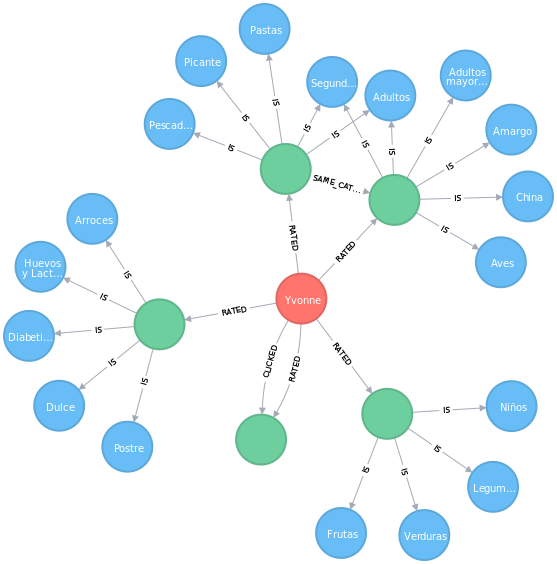
\includegraphics[width=22.5cm,height=12cm]{./images/graph}
            \caption{Modelo de datos implementado para el caso de estudio}
          \end{figure}
          \end{landscape}
        \newpage
